

\chapter{Il controllo attivo di un processo} % (fold)
\label{chap:Il controllo attivo di un processo}

Questa materia si basa sulal premessa che una \textbf{variabile controllata} deve essere
uguale a una \textbf{variabile di riferimento}.

Se il segnale di riferimento è costante, il problema è di \textbf{regolazione}, invece, 
se il segnale di riferimento è variabile, il problema è di \textbf{asservimento}.

\section{Generalità sul concetto di sistema} % (fold)
\label{sec:Generalità sul concetto di sistema}

\begin{theorem}[Sistema]
  \theoremlist{Definizione di sistema}
  Un sistema è un insieme di componenti che interagiscono tra loro,
  in cui si possono distinguere grandezze soggette a variare nel tempo (\textbf{variabili}).
\end{theorem}

\begin{theorem}[Segnale]
  \theoremlist{Definizione di segnale}
  Le funzioni che rappresentano l'andamento delle variabili nel tempo si dicono segnali.
\end{theorem}

Una carrellata di termini:
\begin{itemize}
  \item Variabili controlate(o regolate)
  \item Variabili di riferimento
  \item Variabili manipolabili(o di controllo)
  \item Variabili non manipolabili
  \item Variabili osservate(o misurate)
\end{itemize}

Comunque la distinzione principale che si fa sulle variabili riguarda la lor odipendenza o indipendenza,
cioè se sono variabili di ingresso o di uscita.

\begin{theorem}[Modello matematico]
  \theoremlist{Definizione di Modello matematico}
  Si dice modello matematico (o m.m.) la descrizione di un sistema(con equazioni parametriche e parametri) che permette di ottenere le variabili si uscita

  dalle variabili d'ingresso e di capire quali siano queste variabili d'ingresso.
\end{theorem}

Esisiotno due tipi di modelli matematici:
\begin{itemize}
  \item Sistemi multi-input multi-output (MIMO)
  \item Sistemi single-input single-output (SISO)
\end{itemize}


\begin{theorem}[Sistema statico]
  \theoremlist{Definizione di Sistema statico}

  Un sistema è detto statico (o puramente algebrico) se le variabili di uscita dipendono solo dalle variabili di ingresso al medesimo tempo $t$.

  \begin{equation}
    [\exists f : \Re \rightarrow \Re \ni y(t) = f(u(t)) \quad \forall t \in \Re]
  \end{equation}
\end{theorem}

\begin{theorem}[Sistema dinamico]
  \theoremlist{Definizione di Sistema dinamico}
  Un sistema è detto dinamico quando l'uscita al tempo $t$ dipende dal segnale del'ingresso sull'intervallo $]-\infty, t]$.


  % TODO: AGGIUNGERE LA FORMULA DELLA DEFINIZIONE PER IL SSITEMA DINAMICO
\end{theorem}

Quando si parla di sistemi dinamici, si deve introdurre i concetti di:
\begin{itemize}
  \item Sistema in quiete(o in equilibrio)
  \item Sistema in condizioni asintotiche(o stazionarie)
  \item Sistema a regime
\end{itemize}

\begin{theorem}[Insieme dei behaviors]
  \theoremlist{Definizione di Insieme dei behaviors}
  L'insieme dei behaviors di un sistema è l'insieme delle coppie di segnali ingresso-uscita che possono essere ottenute dal sistema.
\end{theorem}

\begin{theorem}[Linearit\`a]
  \theoremlist{Definizione di Linearit\`a}
  Un sistema si dice lineare quando soddisfa la propriet\`a di sovrapposizione degli effetti:
\end{theorem}

\begin{theorem}[Stazionariet\`a]
  \theoremlist{Definizione di Stazionariet\`a}
  Un sistema si dice stazionario (invariante nel tempo) quando la risposta dell'uscita non dipende dal tempo.
\end{theorem}

% section Generalità sul concetto di sistema (end)

\section{Controllo ad azione diretta e in retroazione}
\subsection{Controllo adazione diretta}
Si ricade nel caso di feedfarward quando l'azione di comando dipende da:
\begin{itemize}
  \item obiettivo perseguito
  \item informazioni sul modello del sistema controllato
  \item disturbi
\end{itemize}

\subsection{Controllo in retroazione}
Il controllo feedback si ha quando l'azione di comando dipende da:
\begin{itemize}
  \item Obiettivo perseguito
  \item Informazioni su modello del sistema di controllo
  \item Disturbi
  \item Variabili controllate
\end{itemize}


\subsection{Confonto tra feedforward e feedback}

\begin{figure}[h!]
  \centering
  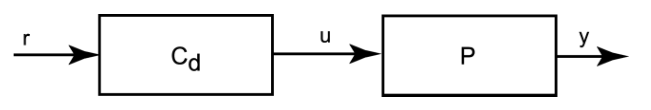
\includegraphics[width=0.5\linewidth]{./images/controllo_azione_diretta.png}
  \caption{Esempio controllo ad azione diretta}
  \label{fig:feedforward}
\end{figure}

Per ottenere il valore dell'uscita:
\begin{align*}
  y &= Pu \\
    &= P(C_dr) \\
    &= PC_dr \\
\end{align*}

Dall'obiettivo so che:
\begin{align*}
  r(t) \equiv y(t) \Rightarrow C_d = \frac{1}{P}
\end{align*}

\begin{figure}[h!]
  \centering
  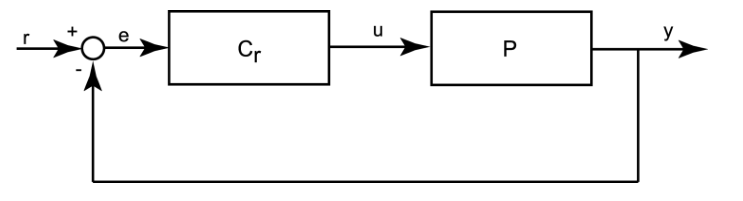
\includegraphics[width=0.5\linewidth]{./images/controllo_retroazione.png}
  \caption{Esempio controllo in retroazione}
  \label{fig:feedback}
\end{figure}

In questo caso l'uscita è data da:
\begin{align*}
  y = \frac{PC_r}{1+PC_r} \cdot r
\end{align*}

Si capisce che l'obiettivo non è raggiungibile e si opta per un obiettivo approssimato:
\begin{align*}
  y(t) \cong r(t) \Rightarrow C_r  >> \frac{1}{P}
\end{align*}

% chapter Il controllo attivo di un processo (end)
